\documentclass[11pt]{article}

\usepackage[margin=1in]{geometry}
\usepackage{amsmath,amssymb}
\usepackage{graphicx}
\usepackage{booktabs}
\usepackage{array}
\usepackage{url}
\usepackage[hidelinks]{hyperref}

\DeclareMathOperator{\sign}{sign}
\DeclareMathOperator*{\argmin}{arg\,min}
\DeclareMathOperator*{\argmax}{arg\,max}

\emergencystretch=3em
\setlength{\parindent}{0pt}
\setlength{\parskip}{0.6em}

\begin{document}

\section{Introduction}

Deep Learning is used in various domains of machine learning (ML): image classification, object recognition, object detection, speech recognition, language translation, voice synthesis, natural language processing. All these applications uses different deep learning techniques like Deep Neural Networks (DNN), Deep Reinforcement Learning (DRL), Federated Machine Learning (FL) and Transfer Learning (TL)~\cite{yuan2019}. Deep learning is proven to give significant progress in these domains. Many of these applications require safety and security failing may result in incorrect results. DNN, DRL, FL and TL techniques are prone to adversarial attacks which result in poor performance. Adversarial attacks pose a serious threat to the success of deep learning in practice. DNNs are vulnerable to towards adversarial attacks that exploit imperceptibly perturbed examples to fool the neural networks. For an instance deliberately crafted adversarial examples can easily deceive DNN based systems such as hand writing recognition, face detection and autonomous vehicle making models generate incorrect outputs. To protect deep learning neural networks from adversarial attacks researchers have been actively developing robust defense mechanisms. These defenses are crucial for ensuring the reliability and security of deep learning applications. some of the ongoing defense strategies for enhancing the robustness of deep learning models are adversarial training, input transformation and architectural modifications which allow real world applications to function effectively without interruptions. This study aims to systematically investigate the evolving landscape of adversarial threats against deep learning models and the defense strategies developed to address these vulnerabilities. The analysis considers a wide range of adversarial attack techniques under diverse threat assumptions, attacker capabilities, and operational scenarios. In contrast to surveys that primarily focus on particular application domains, this work adopts a broader perspective by examining adversarial attacks and corresponding mitigation approaches across multiple deep learning contexts. In addition, the study discusses representative practical examples to demonstrate how these attacks can be realized, how different defense mechanisms respond to them, and the challenges associated with achieving reliable model robustness in practical environments.

This paper presents a comprehensive investigation of adversarial attacks and corresponding defense mechanisms targeting deep learning techniques. To establish a systematic understanding of the research domain, relevant concepts, terminology, and key terms are organized into a structured taxonomy. Furthermore, adversarial threat models are classified based on their characteristics, attacker capabilities, objectives, and underlying attack settings, providing a unified framework for analyzing the security and robustness of deep learning systems.

\section{Background}

\textbf{Taxonomy of Deep Learning Techniques and Adversarial model:}

\paragraph{Deep Neural Network.} The concept of a deep neural network is inspired by biological neural systems. A neural network consists of an interconnected collection of artificial neurons. An individual neuron receives an input vector $x$ through multiple incoming channels, computes an inner product with a weight vector $w$, and passes the result through a non-linear activation function $f(\cdot)$. The output of the neuron is given by $y = f(w^{T}x + b)$. A neural network is formed through the layered interconnection of these processing units.

\begin{figure}[htbp]
  \centering
  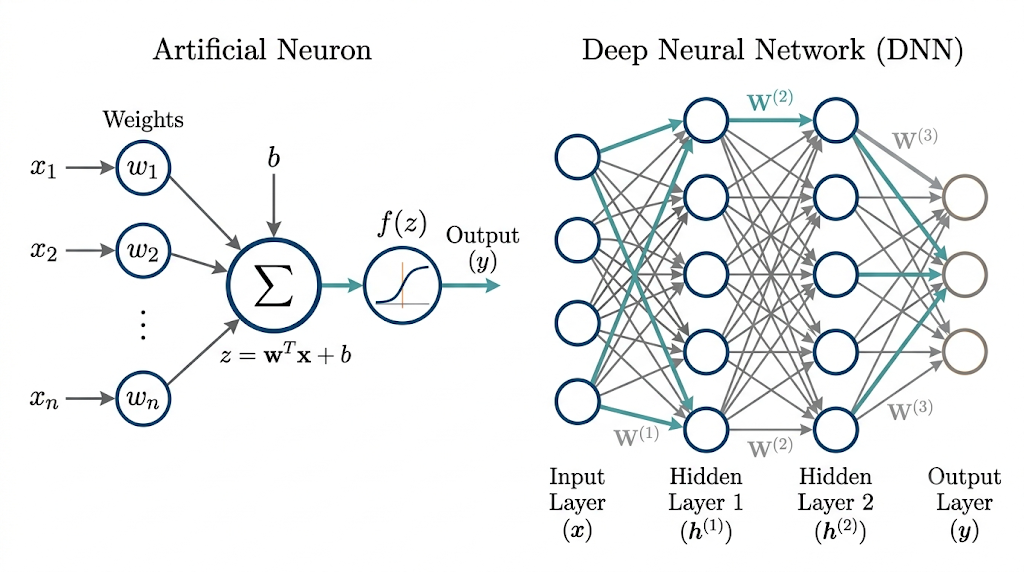
\includegraphics[width=0.95\textwidth]{figures/fig1_neuron_dnn.png}
  \caption{Artificial Neuron and Deep Neural Network.}
  \label{fig:dnn}
\end{figure}

A deep neural network (DNN) takes raw data as input. A DNN comprises an input layer, multiple hidden layers, and an output layer; these intermediate hidden layers hierarchically extract latent features from the raw data. Through these successive layer-wise transformations, the network computes complex mappings to solve challenging real-world problems.

Convolutional Neural Networks (CNNs) are primarily designed to process structured grid data, such as images. A standard CNN architecture comprises convolutional layers, pooling layers, non-linear activation functions, and fully connected layers. Convolutional layers extract hierarchical spatial features from input images, ranging from low-level edges and textures to complex semantic patterns. Pooling layers apply aggregation functions over local spatial regions to downsample feature maps and retain salient activations. Activation functions introduce non-linearity, enabling the network to model complex relationships among extracted features. Finally, one or more fully connected layers map these representations to target predictions, such as classification logits.

\begin{figure}[htbp]
  \centering
  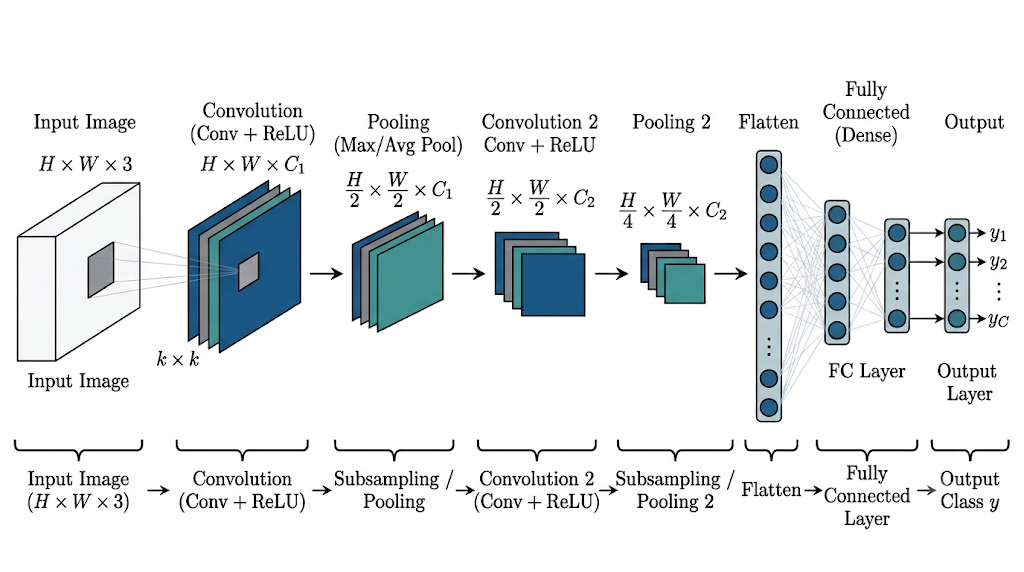
\includegraphics[width=0.95\textwidth]{figures/fig2_cnn.png}
  \caption{Convolutional Neural Network.}
  \label{fig:cnn}
\end{figure}

\paragraph{Federated Learning (FL).} Federated learning (FL) is a machine learning setting where many clients (e.g.\ mobile devices or whole organizations) collaboratively train a model under the orchestration of a central server (e.g.\ service provider), while keeping the training data decentralized. FL embodies the principles of focused data collection and minimization, and can mitigate many of the systemic privacy risks and costs resulting from traditional, centralized machine learning and data science approaches~\cite{kairouz2021}.

\paragraph{Transfer Learning (TL).} Transfer learning is a machine learning paradigm in which knowledge acquired by a model from a source task or domain is leveraged to improve the learning process of a related target task or domain. Instead of developing a model entirely from the beginning, the parameters or feature representations learned from the source task can be adapted to the target problem. This approach is particularly beneficial when the target task has limited labeled training data, as it can reduce the computational cost and training time while improving model generalization and predictive performance. The effectiveness of transfer learning is largely attributed to the reuse of transferable representations that capture features applicable across related tasks or domains.

\paragraph{Deep Reinforcement Learning (DRL).} Deep Reinforcement Learning (DRL) is an AI technique that combines reinforced learning with deep neural networks. It learns to take actions based on feedback in the form of a reward or a penalty signal. This feedback about reward and penalty defines the policy that maximizes the reward function. This policy is represented as the neural network whose input is the current state and output is the probability distribution of possible actions. Inherently reinforced learning is well suited for the application without having a training data set. In deep reinforcement learning, the decision is made based on feedback from the environment.

\section{Adversarial Attacks}

An adversarial attack on deep learning is a technique designed to fool a neural network into making incorrect predictions by applying small, intentionally crafted perturbations to the input data. These attacks significantly decrease the model's performance. Adversarial attacks are intended to undermine the reliability of the model. Adversarial attacks can be systematically categorized along multiple foundational axes, including the adversary's knowledge, operational objectives, and execution timing.

In adversarial machine learning, a threat model defines the precise boundaries, assumptions, and capabilities governing the adversary's interaction with the target system. Standardizing the threat model is critical to ensuring sound evaluation integrity and avoiding artificial claims of robustness~\cite{carlini2019}.

Formally, an adversarial threat model is parameterized along four orthogonal operational axes: Adversary Knowledge, Adversary Goals, Adversary Capabilities and Perturbation Budgets, and Attack Timing.

\subsection{Adversary's Goal}

Based on the adversary's operational objective, adversarial attacks are broadly classified into confidence reduction, untargeted misclassification targeted misclassification and misclassification.

\paragraph{Untargeted Attacks.} The objective of an untargeted attack is to force the model into any incorrect classification, regardless of the resulting output label. For instance, given an image of a cat, the adversary introduces a subtle perturbation such that the model fails to predict the class `cat' and instead outputs an arbitrary incorrect class.

\paragraph{Targeted Attacks.} Targeted attacks aim to force the model to misclassify an input into a specific, predetermined target class different from its true label. For example, the adversary crafts a perturbation such that an image of a cat is predicted not merely as an arbitrary wrong class, but explicitly as a chosen label, such as `dog'.

\paragraph{Confidence Reduction.} Confidence reduction attacks are adversarial perturbations engineered to suppress the prediction confidence of deployed deep learning systems. For instance, in image classification, an adversary crafts subtle input perturbations that drive down the confidence score of the true class or distribute probability mass across alternative categories, significantly impairing the model's decision certainty.

\paragraph{Missclassification.} Misclassification attacks are adversarial perturbations engineered to push input representations across a model's learned decision boundaries, thereby compelling the classifier to assign incorrect output labels to legitimate samples. The objective is to alter the model's prediction to any incorrect class distinct from the original label.

\subsection{Based on Distance Metrics}

In this category of adversarial attacks, the perturbations introduced into the input data are constrained to remain as small as possible while still causing the model to produce incorrect predictions. The magnitude of these perturbations is quantified using different $L_p$ norms, such as the $L_0$, $L_2$, and $L_\infty$ norms. These metrics measure different aspects of the perturbation, including the number of modified features, the overall magnitude of the changes, and the maximum change applied to any individual feature, respectively.

\paragraph{$L_0$ norm.} The $L_0$ norm quantifies sparsity by measuring the total number of input features or pixels altered between the clean and adversarial samples, regardless of the magnitude of each change.

\paragraph{$L_2$ norm.} The $L_2$ norm quantifies the Euclidean distance between the clean and adversarial samples by measuring the square root of the sum of squared differences across all pixel values.

\paragraph{$L_\infty$ norm.} Under the $L_\infty$ norm, the perturbation budget is determined by the maximum absolute deviation across all pixels between the original input and its adversarial counterpart.

\subsection{Adversary's Timing}

\subsubsection{Training-time adversarial capabilities}

Attacks that exploit the training phase, commonly termed causative attacks, are distinguished by the degree of control an adversary exerts over the learning pipeline~\cite{barreno2006,huang2011}. Following the capability-based taxonomy of Papernot et al.~\cite{papernot2018sok}, three levels are generally recognized, in order of increasing strength.

\paragraph{Data Injection.} At the weakest level, an adversary with data injection capability can contribute new samples to the training corpus but has no means of modifying or removing existing records. This situation arises in systems that continually retrain on user-contributed or crawled data, where an attacker may submit maliciously crafted inputs through legitimate channels~\cite{biggio2018}.

\paragraph{Data Modification.} A stronger adversary possesses data modification capability, meaning direct write access to the existing training data or its annotations. Such an attacker may corrupt labels, perturb feature values, or otherwise alter records already in the dataset, which affords finer control over the resulting decision boundary than injection alone~\cite{biggio2012,xiao2015}.

\paragraph{Logic Corruption.} The strongest threat model assumes logic corruption, in which the adversary can interfere with the learning procedure itself, for example by tampering with the training code, the optimization process, or the model parameters. This capability is most relevant to supply-chain settings, such as the use of third-party pretrained models or outsourced training, where the integrity of the learning process cannot be verified by the end user~\cite{papernot2018sok,gu2017}.

\paragraph{Poisoning attacks (Training Time).} Poisoning attacks are executed during the training phase of machine learning models to corrupt the underlying learning process. In this threat model, the adversary injects carefully crafted malicious samples into the training dataset, thereby manipulating the learned parameter set and degrading the generalization performance or integrity of the resulting classifier.

\paragraph{Evasion attacks (Testing Time).} Evasion attacks represent the most prevalent adversarial attack vector and are executed strictly during the inference (testing) phase. In this regime, the adversary crafts deceptive input samples designed to mislead the target model into producing erroneous outputs at runtime. Crucially, the adversary leaves the model parameters, architecture, and underlying training pipeline entirely unaltered, exploiting pre-existing vulnerabilities in the learned decision boundaries.

\subsection{Adversary's Knowledge}

\subsubsection{White Box}

In a white-box attack, the adversary possesses complete knowledge of the target system, including the network architecture, trained weights, and training hyperparameters. By exploiting direct access to the model's loss gradients, the attacker crafts subtle perturbations to input samples that reliably force the classifier into producing erroneous outputs.

\paragraph{Fast Gradient Sign Method (FGSM).} FGSM generates an adversarial image by adding a pixel-wise perturbation of magnitude $\epsilon$ in the direction of the sign of the loss gradient with respect to the input~\cite{goodfellow2015}. Operating as a single-step technique, FGSM achieves high computational efficiency by requiring only a single backward pass to craft the perturbed input.

\subparagraph{Method.} Let $x$ be a clean input with true label $y$, $\theta$ the model parameters, and $J(\theta, x, y)$ the training loss. FGSM takes a single step in the direction that increases the loss, using only the sign of the gradient:
\begin{equation}
  x_{adv} = x + \epsilon \cdot \sign\!\big(\nabla_x J(\theta, x, y)\big)
\end{equation}
Here $\epsilon$ controls the perturbation magnitude. Because the sign operation gives every input dimension a change of exactly $\pm\epsilon$, the perturbation satisfies an $L_\infty$ constraint, $\lVert x_{adv} - x \rVert_\infty \le \epsilon$~\cite{goodfellow2015}. The adversarial example is then typically clipped to the valid input range (e.g., $[0,1]$ for images).

\subparagraph{Key properties.}
\begin{itemize}
  \item \textbf{Efficiency.} Only one gradient computation (one backward pass) is needed, making FGSM much cheaper than iterative optimization-based attacks such as the L-BFGS formulation in~\cite{szegedy2014}.
  \item \textbf{White-box requirement.} The attacker needs access to the model's gradients, so FGSM is a white-box attack.
  \item \textbf{Untargeted by default.} The basic form maximizes the loss on the true label. A targeted variant instead minimizes the loss with respect to a chosen target label, taking a step in the negative gradient direction.
  \item \textbf{Transferability.} Adversarial examples crafted on one model often fool others, which enables black-box attacks using a surrogate model~\cite{goodfellow2015,papernot2016transfer}.
  \item \textbf{Use in defense.} Goodfellow et al.\ also proposed using FGSM examples during training (adversarial training) as a regularizer to improve robustness~\cite{goodfellow2015}.
\end{itemize}

For a targeted attack, the same method is applied, with the key difference being that the perturbation is generated in the direction of the negative gradient of the loss with respect to the target class, encouraging the model to classify the input as the desired target class~\cite{li2020}.
\begin{equation}
  x_{adv} = x - \epsilon \cdot \sign\!\big(\nabla_x J(\theta, x, y_t)\big)
\end{equation}
where:
\begin{itemize}
  \item $x_{adv}$ --- generated adversarial example.
  \item $x$ --- original input.
  \item $\epsilon$ --- perturbation magnitude.
  \item $J(\theta, x, y_t)$ --- loss function evaluated with respect to the target class $y_t$.
  \item $\nabla_x J(\theta, x, y_t)$ --- gradient of the loss with respect to the input.
  \item $\sign(\cdot)$ --- sign function applied to each gradient component.
  \item $y_t$ --- desired target class.
\end{itemize}

\paragraph{Projected Gradient Descent (PGD).} PGD is one of the most popular and widely used white-box attacks~\cite{madry2018}. It is an iterative extension of FGSM: at each step, the input is perturbed in the direction of the sign of the loss gradient, and the result is then projected back onto the allowed perturbation set (e.g., an $L_\infty$ ball of radius $\epsilon$ around the original input) so that the perturbation budget is never exceeded~\cite{madry2018,kurakin2017}. PGD is typically initialized at a random point within this ball. Because it is not restricted to a single step, it can spend as much computation as needed, and it is therefore considered a much stronger attack than FGSM. The process is repeated until the attack succeeds (i.e., the model's predicted class changes) or a fixed number of iterations is reached.

\subparagraph{PGD update equation.} For an untargeted PGD attack under an $L_\infty$ constraint, the iterative update is expressed as:
\begin{equation}
  x^{t+1} = \Pi_{x+\mathcal{S}}\!\Big(x^{t} + \alpha \cdot \sign\!\big(\nabla_x J(\theta, x^{t}, y)\big)\Big)
\end{equation}
where:
\begin{itemize}
  \item $x$ is the original, clean input.
  \item $x^{(t)}$ is the adversarial input at iteration $t$.
  \item $x^{(t+1)}$ is the updated adversarial input.
  \item $\alpha$ is the step size used at each iteration.
  \item $J(\theta, x^{(t)}, y)$ is the loss function evaluated at the current input.
  \item $\nabla_{x^{(t)}} J$ is the gradient of the loss with respect to the current input.
  \item $\Pi_{x+\mathcal{S}}$ denotes projection onto the allowed perturbation region centered at the original input.
  \item $\sign(\cdot)$ determines the direction of each input update.
\end{itemize}
The equation above follows the standard $L_\infty$-constrained PGD formulation described by Madry et al.~\cite{madry2018}.

\paragraph{DeepFool.} DeepFool is an untargeted, iterative white-box attack proposed by Moosavi-Dezfooli et al.~\cite{moosavi2016} that generates minimal adversarial perturbations based on the geometry of the classifier's decision boundaries. Instead of maximizing loss within a pre-allocated perturbation budget like FGSM or PGD, DeepFool computes the minimal perturbation required to push an input across the closest decision boundary.

To formalize this concept, consider an affine binary classifier:
\begin{equation}
  f(x) = w^{T}x + b
\end{equation}
where the decision boundary corresponds to the hyperplane $F = \{x : w^{T}x + b = 0\}$. The exact minimal perturbation $\delta^{*}(x)$ required to alter the classification corresponds to the orthogonal projection of $x$ onto $F$:
\begin{equation}
  \delta^{*}(x) = -\frac{f(x)}{\lVert w \rVert_2^{2}}\, w
\end{equation}
Because deep neural networks are non-linear, their decision boundaries are represented by complex, non-linear hyper-surfaces. DeepFool addresses this by iteratively linearizing the boundary around the current iterate $x_i$ using a first-order Taylor approximation:
\begin{equation}
  f(x) \approx f(x_i) + \nabla f(x_i)^{T}(x - x_i)
\end{equation}
In a multi-class setting with $C$ classes, the algorithm computes the projection onto the closest separating hyperplane among all alternative classes $k \neq \hat{k}(x)$.
% NOTE: the source document breaks off here with a colon; the multi-class
% projection equation it introduces is missing from the source.
The perturbation vector is accumulated iteratively until the input crosses the boundary, yielding tighter $L_2$ and $L_\infty$ perturbation bounds and serving as an accurate empirical proxy for classifier robustness~\cite{moosavi2016}.

\paragraph{Carlini and Wagner (C\&W) Attacks.} Carlini and Wagner introduced a suite of optimization-based adversarial attacks designed to evaluate the limits of adversarial robustness~\cite{carlini2017}. Specifically developed to defeat defensive distillation~\cite{papernot2016distill} and other heuristic defenses that rely on gradient masking, the C\&W framework formulates adversarial example generation as a constrained, continuous optimization problem rather than a greedy gradient-ascent heuristic.

\subparagraph{Optimization Formulation.} Given an input $x \in \mathbb{R}^d$, the objective is to synthesize a perturbation $\delta$ of minimum norm that forces a neural network $f(\cdot)$ to predict a chosen target class $t \neq y$, while satisfying the box constraint that the perturbed sample remains a valid image ($x + \delta \in [0,1]^d$). Carlini and Wagner expressed this constrained problem as:
\begin{equation}
  \min_{\delta}\ \lVert \delta \rVert_p + c \cdot g(x+\delta) \quad \text{subject to} \quad x + \delta \in [0,1]^d
\end{equation}
where:
\begin{itemize}
  \item $\lVert \cdot \rVert_p$ denotes the chosen $L_p$ distance metric, predominantly instantiated under the $L_0$, $L_2$, or $L_\infty$ norm.
  \item $c > 0$ is a dynamically tuned regularization constant determined via binary search.
  \item $g(\cdot)$ is an objective loss function engineered such that $g(x+\delta) \le 0$ if and only if the model predicts the target class $t$.
\end{itemize}

\subparagraph{Logit-Based Objective Function ($g$).} To prevent the vanishing gradient issues caused by standard saturated softmax cross-entropy losses---which defensive distillation inherently exploits---Carlini and Wagner evaluated several candidate objective functions and identified the logit-difference loss as the most effective:
\begin{equation}
  g(x') = \max\!\Big(\max_{i \neq t} Z(x')_i - Z(x')_t,\; -\kappa\Big)
\end{equation}
where:
\begin{itemize}
  \item $Z(x')_i$ represents the unnormalized logit score corresponding to class $i$ prior to the softmax activation layer.
  \item $\kappa \ge 0$ denotes a confidence parameter. Setting $\kappa = 0$ yields a minimal perturbation that marginally flips the prediction, whereas $\kappa > 0$ crafts high-confidence adversarial examples that exhibit enhanced transferability across distinct architectures.
\end{itemize}

\subparagraph{Box-Constraint Handling: Change of Variables.} To eliminate the need for projected gradient descent or heuristic clipping when enforcing $x + \delta \in [0,1]^d$, C\&W introduced a change-of-variables formulation using the hyperbolic tangent function:
\begin{equation}
  \delta_i = \tfrac{1}{2}\big(\tanh(w_i) + 1\big) - x_i
\end{equation}
Under this transformation, any unconstrained real-valued parameter vector $w \in \mathbb{R}^d$ inherently satisfies:
\begin{equation}
  0 \le x_i + \delta_i = \tfrac{1}{2}\big(\tanh(w_i) + 1\big) \le 1
\end{equation}
This allows the optimization problem to be solved smoothly using standard unconstrained gradient-based optimizers, such as Adam~\cite{kingma2015}.

\subparagraph{Attack Variants Across Norms.} Carlini and Wagner instantiated their framework across three standard distance metrics:
\begin{itemize}
  \item \textbf{$L_2$ Attack:} Optimizes $\lVert \delta \rVert_2^{2} + c \cdot g(x+\delta)$ directly using the Adam optimizer, generating perturbations with significantly lower Euclidean distortion than FGSM or DeepFool.
  \item \textbf{$L_\infty$ Attack:} Employs an iterative penalty method to minimize $\max_i \lvert \delta_i \rvert$, penalizing only the dimensions that exceed a progressively decaying threshold $\tau$.
  \item \textbf{$L_0$ Attack:} An iterative greedy algorithm that uses the $L_2$ attack to identify non-critical coordinates, iteratively masking out pixels that contribute least to the adversarial objective until a minimal subset remains.
\end{itemize}

\paragraph{Jacobian-based Saliency Map Attack (JSMA).} Introduced by Papernot et al.~\cite{papernot2016limitations}, JSMA is a targeted, white-box attack optimized under the $L_0$ norm to alter a minimal number of input features. Rather than computing loss gradients via backpropagation, JSMA evaluates the forward derivative of the network $F(x)$ via its Jacobian matrix $J_F(x) \in \mathbb{R}^{K \times d}$:
\begin{equation}
  J_F(x) = \left[ \frac{\partial F_j(x)}{\partial x_i} \right]_{j \in \{1,\dots,K\},\; i \in \{1,\dots,d\}}
\end{equation}

\subparagraph{Saliency Map and Feature Selection.} To drive the network toward a designated target class $t$, an adversarial saliency map $S(x, t)$ scores each feature $i$ based on its ability to increase the target probability while suppressing competing outputs:
\begin{equation}
  S(x, t)[i] =
  \begin{cases}
    0, & \text{if } \dfrac{\partial F_t(x)}{\partial x_i} < 0 \\[1.5ex]
       & \text{or } \displaystyle\sum_{j \neq t} \dfrac{\partial F_j(x)}{\partial x_i} > 0 \\[1.5ex]
    \dfrac{\partial F_t(x)}{\partial x_i} \left\lvert \displaystyle\sum_{j \neq t} \dfrac{\partial F_j(x)}{\partial x_i} \right\rvert, & \text{otherwise}
  \end{cases}
\end{equation}
The algorithm iteratively selects the highest-scoring pixel pair, saturating their values until $\argmax_j F_j(x_{adv}) = t$ or the sparsity budget $\lVert\delta\rVert_0 \le \gamma \cdot d$ is reached. Due to its $\mathcal{O}(d^2)$ pairwise Jacobian complexity, JSMA scales poorly to high-dimensional datasets~\cite{papernot2018sok,papernot2016limitations}.

\paragraph{Universal Adversarial Perturbations (UAP).} Proposed by Moosavi-Dezfooli et al.~\cite{moosavi2017}, a Universal Adversarial Perturbation (UAP) is a single, input-agnostic noise vector $v \in \mathbb{R}^d$ that misleads a classifier across almost all inputs sampled from a data distribution $\mu$.

\subparagraph{Mathematical Formulation.} The adversary seeks a single perturbation $v$ bounded by an $L_p$ budget $\xi$ that achieves a target fooling rate $1-\delta$:
\begin{equation}
  \lVert v \rVert_p \le \xi \quad \text{such that} \quad \mathbb{P}_{x \sim \mu}\big(\hat{k}(x+v) \neq \hat{k}(x)\big) \ge 1 - \delta
\end{equation}
where $\hat{k}(x)$ denotes the model's predicted label.

\subparagraph{Algorithmic Mechanism.} Initialized at $v = 0$, the algorithm iteratively loops over training samples $x_i \in X$:
\begin{enumerate}
  \item If $\hat{k}(x_i + v) = \hat{k}(x_i)$, it computes the minimal additional perturbation $\Delta v_i$ required to cross the decision boundary (typically via DeepFool~\cite{moosavi2016}):
  \begin{equation}
    \Delta v_i = \argmin_{r} \lVert r \rVert_2 \quad \text{s.t.} \quad \hat{k}(x_i + v + r) \neq \hat{k}(x_i)
  \end{equation}
  \item The vector is updated and projected back into the $L_p$ ball of radius $\xi$:
  \begin{equation}
    v \leftarrow \Pi_{p,\xi}(v + \Delta v_i)
  \end{equation}
\end{enumerate}
This loop repeats until the empirical fooling rate on $X$ meets or exceeds $1-\delta$. UAPs generalize well across training subsets and exhibit strong cross-architecture transferability~\cite{moosavi2017}.

\subsubsection{Black Box: Operational Taxonomy of Black-Box Attacks}

In adversarial machine learning, black-box threat models are defined along two primary axes: the temporal nature of adversary-target interaction (open-loop vs.\ closed-loop) and the degree of defense awareness and adaptability exhibited by the adversary~\cite{chakraborty2018,carlini2019}. While early surveys categorized black-box attacks primarily by output granularity (score-based vs.\ decision-based)~\cite{chakraborty2018}, practical security audits require a taxonomy organized by operational dynamics.

We formalize three operational regimes: Non-Adaptive Black-Box, Adaptive Black-Box, and Strict Black-Box (No-Box) attacks.

\paragraph{Comparative Operational Taxonomy.}

\begin{table}[htbp]
  \centering
  \small
  \renewcommand{\arraystretch}{1.3}
  \begin{tabular}{@{}>{\raggedright\arraybackslash}p{0.12\textwidth}
                    >{\raggedright\arraybackslash}p{0.16\textwidth}
                    >{\raggedright\arraybackslash}p{0.15\textwidth}
                    >{\raggedright\arraybackslash}p{0.25\textwidth}
                    >{\raggedright\arraybackslash}p{0.19\textwidth}@{}}
    \toprule
    Attack Paradigm & Target Interaction \& Query Budget & Defense Awareness & Optimization Mechanism & Canonical References \\
    \midrule
    Non-Adaptive Black-Box & Open-loop; zero online queries ($Q = 0$) & Oblivious to runtime defenses & Transferability via surrogate landscapes; input transformations; momentum & Papernot et al.~\cite{papernot2017}, Dong et al.~\cite{dong2018}, Xie et al.~\cite{xie2019} \\
    Adaptive Black-Box & Closed-loop; sequential queries ($Q \in [10^2, 10^5]$) & Actively circumvents runtime mitigations & Zeroth-order gradient estimation (NES); boundary tracking; score-based random search & Carlini et al.~\cite{carlini2019}, Athalye et al.~\cite{athalye2018}, Andriushchenko et al.~\cite{andriushchenko2020} \\
    Strict Black-Box (No-Box) & Extreme query constraints ($Q \to 0$); hard labels & Zero parameter, architectural, or distribution knowledge & Synthetic dataset distillation; unsupervised proxy surrogates; topological graph probing & Gao et al.~\cite{gao2022}, Li et al.~\cite{li2020nobox} \\
    \bottomrule
  \end{tabular}
  \caption{Comparative operational taxonomy of black-box attacks.}
  \label{tab:blackbox}
\end{table}

\paragraph{Non-Adaptive Black-Box Attacks.} A non-adaptive black-box attack executes under an open-loop regime: candidate perturbations are generated entirely offline without runtime feedback or iterative refinement against the victim model $f_\theta$~\cite{papernot2017}.

\subparagraph{Operational Characteristics.}
\begin{itemize}
  \item \textbf{Surrogate-Driven Optimization:} The adversary optimizes a bounded perturbation $\delta$ against a locally trained substitute model $\hat{f}_\Phi$ (or an ensemble of heterogeneous architectures $\sum_{m=1}^{M} w_m \hat{f}_{\Phi_m}$):
  \begin{equation}
    \delta^{*} = \argmax_{\lVert\delta\rVert_p \le \epsilon} L\big(\hat{f}_\Phi(x+\delta), y\big)
  \end{equation}
  The resulting adversarial sample $x_{adv} = x + \delta^{*}$ is submitted directly to the target system $f_\theta$ under the assumption of cross-model transferability~\cite{papernot2017,dong2018}.
  \item \textbf{Landscape Stabilization:} Because the adversary cannot verify whether an attack settles into narrow, surrogate-specific loss minima, non-adaptive attacks apply momentum accumulation to stabilize update trajectories across iterations. Dong et al.~\cite{dong2018} formalized Momentum Iterative Fast Gradient Sign Method (MI-FGSM):
  \begin{equation}
    g_{t+1} = \mu \cdot g_t + \frac{\nabla_x L(\hat{f}_\Phi(x_t), y)}{\lVert \nabla_x L(\hat{f}_\Phi(x_t), y) \rVert_1}, \qquad x_{t+1} = \Pi_{x+\mathcal{S}}\big(x_t + \alpha \cdot \sign(g_{t+1})\big)
  \end{equation}
  \item \textbf{Input Diversity Transformations:} To prevent spatial overfitting to the surrogate architecture, Xie et al.~\cite{xie2019} introduced the Diverse Inputs Method (DIM), which applies stochastic image transformations $T(x; p)$ (random resizing and padding with probability $p$) during backpropagation:
  \begin{equation}
    \delta^{*} = \argmax_{\lVert\delta\rVert_p \le \epsilon} \mathbb{E}_T\Big[L\big(\hat{f}_\Phi(T(x+\delta)), y\big)\Big]
  \end{equation}
  \item \textbf{Absence of Runtime Compensation:} Non-adaptive perturbations cannot dynamically compensate for non-deterministic or reactive defense mechanisms (e.g., stochastic input transformation, feature quantization, or test-time noise injection) deployed by the target model.
\end{itemize}

\paragraph{Adaptive Black-Box Attacks.} In an adaptive black-box attack, the adversary interacts with the victim in a closed-loop feedback system. The perturbation evolves sequentially based on observed oracle responses, and the optimization strategy explicitly accounts for defensive countermeasures deployed on the target model~\cite{carlini2019,athalye2018}.

\subparagraph{Operational Characteristics.}
\begin{itemize}
  \item \textbf{Interactive Query Feedback:} The attacker formulates subsequent input queries conditioned on previous model outputs:
  \begin{equation}
    x^{(t+1)} = x^{(t)} + u\Big(\big\{x^{(\tau)}, f_\theta(x^{(\tau)})\big\}_{\tau=1}^{t}\Big), \quad \text{s.t.} \quad \lVert x^{(t+1)} - x \rVert_p \le \epsilon
  \end{equation}
  where $u(\cdot)$ represents a zeroth-order update rule, evolutionary strategy, or geometric boundary adjustment.
  \item \textbf{Circumvention of Obfuscated Gradients:} Athalye et al.~\cite{athalye2018} and Carlini et al.~\cite{carlini2019} demonstrated that defenses relying on gradient masking (shattered gradients, stochastic transformations, or numerical saturation) give a false sense of security. Adaptive adversaries tailor their probing mechanism to bypass these defenses:
  \begin{itemize}
    \item \textbf{Stochastic Defenses:} Mitigated by combining Natural Evolutionary Strategies (NES) with Expectation Over Transformation (EOT), taking expectations over runtime defense transformations:
    \begin{equation}
      \nabla_x \mathbb{E}_{t \sim T}\big[L(f_\theta(t(x)), y)\big] \approx \frac{1}{B\sigma} \sum_{i=1}^{B} \delta_i\, L\big(f_\theta(t(x+\delta_i)), y\big)
    \end{equation}
    \item \textbf{Shattered / Discontinuous Surfaces:} Mitigated by gradient-free exploration methods. Andriushchenko et al.~\cite{andriushchenko2020} designed Square Attack, a score-based search algorithm that updates localized, square-shaped coordinate slices via randomized sampling:
    \begin{equation}
      x^{(t+1)} = \Pi_{x+\mathcal{S}}\big(x^{(t)} + \Delta^{(t)}\big)
    \end{equation}
  \end{itemize}
  \item[] Because Square Attack does not rely on local loss gradients or their numerical approximations, it renders gradient obfuscation defenses ineffective~\cite{carlini2019,andriushchenko2020}.
  \item \textbf{High Query Consumption:} Adaptive optimization requires query access scales typically ranging from $Q \sim 10^2$ (for random-search score attacks~\cite{andriushchenko2020}) to $Q \sim 10^5$ (for hard-label decision-boundary tracking).
\end{itemize}

\paragraph{Strict Black-Box Attacks (No-Box / Zero-Knowledge).} A strict black-box attack (often designated as a No-Box or Zero-Knowledge threat model~\cite{gao2022,li2020nobox}) represents the most constrained operational setting. It strips away conventional academic relaxations---such as access to identical training data distributions, unlimited query budgets, and continuous logit vectors.

\subparagraph{Operational Characteristics.}
\begin{itemize}
  \item \textbf{Severe Query and Interface Constraints ($Q \to 0$):} The adversary faces aggressive query rate-limiting, CAPTCHAs, or active stateful query analyzers that prevent the multi-thousand query iterations required by zeroth-order methods~\cite{carlini2019,andriushchenko2020}. The model provides only hard, discrete top-1 predictions:
  \begin{equation}
    \hat{y} = \argmax_{c \in \{1, \dots, K\}} f_\theta(x)_c
  \end{equation}
  \item \textbf{Distributional and Architectural Disparity:} Unlike the assumptions in Papernot et al.~\cite{papernot2017}, the adversary possesses neither the target model's training dataset $D_{train}$ nor architectural knowledge (e.g., whether the victim is a ResNet, a Vision Transformer, or an ensemble). Li et al.~\cite{li2020nobox} formalize practical no-box attacks where the attacker trains generative networks or surrogate models using uncurated, out-of-domain public data or self-supervised feature reconstructors without target feedback.
  \item \textbf{Non-Euclidean and Domain Extensions:} Strict black-box threat models extend beyond Euclidean continuous manifolds into discrete, structured topologies. Gao et al.~\cite{gao2022} demonstrated strict black-box adversarial attacks on Graph Neural Networks (GNNs), where attackers modify graph structures (node features and edge connectivity) with zero victim query feedback and restricted topological visibility:
  \begin{equation}
    \max_{A' \in V_{budget}} L_{GNN}\big(f_\theta(A', X), Y\big)
  \end{equation}
  showing that topological vulnerabilities can be exploited without model access or interactive feedback.
\end{itemize}

\begin{thebibliography}{99}

\bibitem{yuan2019} X. Yuan, P. He, Q. Zhu, and X. Li, ``Adversarial examples: Attacks and defenses for deep learning,'' \textit{IEEE Transactions on Neural Networks and Learning Systems}, vol. 30, no. 9, pp. 2805--2824, Sep. 2019, doi: 10.1109/TNNLS.2018.2886017.

\bibitem{kairouz2021} P. Kairouz et al., ``Advances and open problems in federated learning,'' \textit{Foundations and Trends in Machine Learning}, vol. 14, nos. 1--2, pp. 1--210, 2021, doi: 10.1561/2200000083.

\bibitem{carlini2019} N. Carlini, A. Athalye, N. Papernot, W. Brendel, J. Rauber, D. Tsipras, I. Goodfellow, A. Madry, and A. Kurakin, ``On evaluating adversarial robustness,'' arXiv preprint arXiv:1902.06705, 2019.

\bibitem{barreno2006} M. Barreno, B. Nelson, R. Sears, A. D. Joseph, and J. D. Tygar, ``Can machine learning be secure?,'' in \textit{Proc. 2006 ACM Symp. on Information, Computer and Communications Security (ASIACCS '06)}, Taipei, Taiwan, Mar. 2006, pp. 16--25, doi: 10.1145/1128817.1128824.

\bibitem{huang2011} L. Huang, A. D. Joseph, B. Nelson, B. I. P. Rubinstein, and J. D. Tygar, ``Adversarial machine learning,'' in \textit{Proc. 4th ACM Workshop Secur. Artif. Intell. (AISec)}, 2011, pp. 43--58.

\bibitem{papernot2018sok} N. Papernot, P. McDaniel, A. Sinha, and M. Wellman, ``SoK: Security and privacy in machine learning,'' in \textit{Proc. IEEE Eur. Symp. Security Privacy (EuroS\&P)}, 2018, pp. 399--414.

\bibitem{biggio2018} B. Biggio and F. Roli, ``Wild patterns: Ten years after the rise of adversarial machine learning,'' \textit{Pattern Recognit.}, vol. 84, pp. 317--331, Dec. 2018.

\bibitem{biggio2012} B. Biggio, B. Nelson, and P. Laskov, ``Poisoning attacks against support vector machines,'' in \textit{Proc. 29th Int. Conf. Mach. Learn. (ICML)}, 2012.

\bibitem{xiao2015} H. Xiao, B. Biggio, B. Nelson, H. Xiao, C. Eckert, and F. Roli, ``Support vector machines under adversarial label contamination,'' \textit{Neurocomputing}, vol. 160, pp. 53--62, Jul. 2015.

\bibitem{gu2017} T. Gu, B. Dolan-Gavitt, and S. Garg, ``BadNets: Identifying vulnerabilities in the machine learning model supply chain,'' arXiv:1708.06733, 2017.

\bibitem{goodfellow2015} I. J. Goodfellow, J. Shlens, and C. Szegedy, ``Explaining and harnessing adversarial examples,'' in \textit{Proc. Int. Conf. Learn. Represent. (ICLR)}, San Diego, CA, USA, 2015. [Online]. Available: \url{https://arxiv.org/abs/1412.6572}

\bibitem{szegedy2014} C. Szegedy et al., ``Intriguing properties of neural networks,'' in \textit{Proc. Int. Conf. Learn. Represent. (ICLR)}, 2014. arXiv:1312.6199.

\bibitem{papernot2016transfer} N. Papernot, P. McDaniel, and I. Goodfellow, ``Transferability in machine learning: From phenomena to black-box attacks using adversarial samples,'' arXiv:1605.07277, 2016.

\bibitem{li2020} Y. Li and Y. Liu, ``Adversarial attacks and defenses in deep learning,'' \textit{Engineering}, vol. 6, no. 3, pp. 346--360, Mar. 2020, doi: 10.1016/j.eng.2019.12.012.

\bibitem{madry2018} A. Madry, A. Makelov, L. Schmidt, D. Tsipras, and A. Vladu, ``Towards deep learning models resistant to adversarial attacks,'' in \textit{Proc. Int. Conf. Learn. Represent. (ICLR)}, 2018. [Online]. Available: \url{https://arxiv.org/abs/1706.06083}

\bibitem{kurakin2017} A. Kurakin, I. Goodfellow, and S. Bengio, ``Adversarial examples in the physical world,'' in \textit{Proc. Int. Conf. Learn. Represent. (ICLR) Workshop}, 2017. [Online]. Available: \url{https://arxiv.org/abs/1607.02533}

\bibitem{moosavi2016} S.-M. Moosavi-Dezfooli, A. Fawzi, and P. Frossard, ``DeepFool: A simple and accurate method to fool deep neural networks,'' in \textit{Proc. IEEE Conf. Comput. Vis. Pattern Recognit. (CVPR)}, Las Vegas, NV, USA, 2016, pp. 2574--2582.

\bibitem{carlini2017} N. Carlini and D. Wagner, ``Towards evaluating the robustness of neural networks,'' in \textit{Proc. IEEE Symp. Secur. Privacy (SP)}, San Jose, CA, USA, 2017, pp. 39--57.

\bibitem{papernot2016distill} N. Papernot, P. McDaniel, X. Wu, S. Jha, and A. Swami, ``Distillation as a defense to adversarial perturbations against deep neural networks,'' in \textit{Proc. IEEE Symp. Secur. Privacy (SP)}, San Jose, CA, USA, 2016, pp. 582--597.

\bibitem{kingma2015} D. P. Kingma and J. Ba, ``Adam: A method for stochastic optimization,'' in \textit{Proc. Int. Conf. Learn. Representations (ICLR)}, San Diego, CA, USA, 2015, pp. 1--15.

\bibitem{papernot2016limitations} N. Papernot, P. McDaniel, S. Jha, M. Fredrikson, Z. B. Celik, and A. Swami, ``The limitations of deep learning in adversarial settings,'' in \textit{Proc. 1st IEEE Eur. Symp. Secur. Privacy (EuroS\&P)}, 2016, pp. 372--387.

\bibitem{moosavi2017} S.-M. Moosavi-Dezfooli, A. Fawzi, O. Fawzi, and P. Frossard, ``Universal adversarial perturbations,'' in \textit{Proc. IEEE Conf. Comput. Vis. Pattern Recognit. (CVPR)}, 2017, pp. 1765--1773.

\bibitem{chakraborty2018} A. Chakraborty, M. Alam, V. Dey, A. Chattopadhyay, and D. Mukhopadhyay, ``Adversarial attacks and defences: A survey,'' arXiv preprint arXiv:1810.00069, 2018.

\bibitem{papernot2017} N. Papernot, P. McDaniel, I. Goodfellow, S. Jha, Z. B. Celik, and A. Swami, ``Practical black-box attacks against machine learning,'' in \textit{Proc. ACM Asia Conf. Comput. Commun. Secur. (ASIACCS)}, 2017, pp. 506--519.

\bibitem{dong2018} Y. Dong, F. Liao, T. Pang, H. Su, J. Zhu, X. Hu, and J. Li, ``Boosting adversarial attacks with momentum,'' in \textit{Proc. IEEE/CVF Conf. Comput. Vis. Pattern Recognit. (CVPR)}, 2018, pp. 9185--9193.

\bibitem{xie2019} C. Xie, Z. Zhang, Y. Zhou, S. Bai, J. Wang, Z. Ren, and A. L. Yuille, ``Improving transferability of adversarial examples with input diversity,'' in \textit{Proc. IEEE/CVF Conf. Comput. Vis. Pattern Recognit. (CVPR)}, 2019, pp. 2730--2739.

\bibitem{athalye2018} A. Athalye, N. Carlini, and D. Wagner, ``Obfuscated gradients give a false sense of security: Circumventing defenses to adversarial examples,'' in \textit{Proc. Int. Conf. Mach. Learn. (ICML)}, 2018, pp. 274--283.

\bibitem{andriushchenko2020} M. Andriushchenko, F. Croce, N. Flammarion, and M. Hein, ``Square Attack: A query-efficient black-box adversarial attack via random search,'' in \textit{Proc. Eur. Conf. Comput. Vis. (ECCV)}, 2020, pp. 484--501.

\bibitem{gao2022} J. Gao, M. Ding, B. Du, and H. Shen, ``Strict black-box adversarial attacks on graphs,'' in \textit{Proc. AAAI Conf. Artif. Intell. (AAAI)}, vol. 36, no. 1, 2022, pp. 62--70.

\bibitem{li2020nobox} Q. Li, Y. Guo, H. Zha, and H. Chen, ``Practical no-box adversarial attacks against deep neural networks,'' in \textit{Proc. IEEE/CVF Conf. Comput. Vision Pattern Recognit. (CVPR)}, 2020.

\end{thebibliography}

\end{document}
